\lstset{style=sql, basicstyle=\ttfamily\scriptsize}

\title[Datenbanken] {Datenbanken und SQL}

\date[\today] % (optional)

\logo{\includegraphics[width=.8cm]{Logos/FreeFlower.pdf}}

\frame{\titlepage}

\begin{frame}{Einführung}
  \begin{columns}
    \begin{column}{0.6\textwidth}
      \begin{figure}[H]
        \centering
        \includegraphics[height=3.2cm]{Grundlagen_Info/06_Datenbanken/Figures/db-ex1}
        \pause
        \includegraphics[height=3.2cm]{Grundlagen_Info/06_Datenbanken/Figures/db-ex4}
        \pause
        % fiktive Profilkarte im Stil eines sozialen Netzwerks (statt Screenshot eines echten Profils)
        \begin{tikzpicture}
          \node[draw=black!30, fill=white, drop shadow, inner sep=4pt, align=left, text width=.62\columnwidth, font=\tiny] {
            {\scriptsize\textbf{Alex Muster}}\\
            Informatiklehrperson | Datenbanken, Python\\
            \textcolor{gray}{Zürich, Schweiz \textbullet{} Kontaktinfo}\\
            \textcolor{RoyalBlue}{\textbf{700 Follower \textbullet{} 500+ Kontakte}}
          };
        \end{tikzpicture}
        \pause
        \includegraphics[width=.7\columnwidth]{Grundlagen_Info/06_Datenbanken/Figures/db-ex3}

        {\tiny Screenshots: galaxus.ch, Apple Music, sbb.ch; Profil: fiktives Beispiel}
      \end{figure}
    \end{column}
    \pause
    \begin{column}{0.4\textwidth}
      Daten sind omnipräsent...
      \begin{itemize}[<+->]
        \item \textbf{Social Media}: Instagram, TikTok, LinkedIn, etc...
        \item \textbf{Shopping}: Galaxus, AliExpress, etc...
        \item \textbf{Netzwerke}: SBB, swissgrid (Strom-Netzwerk), etc...
      \end{itemize}
      \pause
      Wie können wir mit den riesigen Datenmengen umgehen und sinnvolle Einsichten daraus gewinnen?
    \end{column}
  \end{columns}
\end{frame}

\begin{frame}{Datenmengen und Speicherplatz}
  % Please add the following required packages to your document preamble:
  \centering
  \scriptsize
  Ein \textbf{B}yte = 8 \textbf{b}it
  \begin{table}[H]
    \begin{tabular}{@{}lrrl@{}}
      \toprule
      \textbf{Masseinheit} & \multicolumn{2}{l}{\textbf{Dezimalsystem}} & Grössenordnung                                   \\ \midrule
      kB (Kilobyte)        & $10^3$ B(yte)                               & 1'000 B             & Eine Text-Datei            \\
      MB (Megabyte)        & $10^6$ B                                    & 1'000'000 B         & Eine Musik-Datei           \\
      GB (Gigabyte)        & $10^9$ B                                    & 1'000'000'000 B     & Eine Video-Datei           \\
      TB (Terabyte)        & $10^{12}$ B                                 & 1'000'000'000'000 B & Kleiner Firmen-Server      \\
      PB (Petabyte)        & $10^{15}$ B                                 & ...                 & CERN-Rechenzentrum pro Tag \\
      EB (Exabyte)         & $10^{18}$ B                                 & ...                 & Festplatten des CERN (2023) \\
      ZB (Zettabyte)       & $10^{21}$ B                                 & ...                 & Weltweit pro Jahr (2024: 173 ZB) \\
      YB (Yottabyte)       & $10^{24}$ B                                 & ...                 & Noch nicht erreicht        \\ \bottomrule
    \end{tabular}
  \end{table}
  {\tiny Quellen: CERN (home.cern, abgerufen am 22.11.2026), IDC via Statista (siehe nächste Folie)}
\end{frame}

% \begin{frame}{Soziale Netzwerke}
%  \centering
%  \url{https://youtu.be/_r97qdyQtIk?t=2m14s}
% \end{frame}

\begin{frame}{Entwicklung der globalen Datenmenge}{Pro Jahr erzeugte, kopierte und genutzte Daten (2029: Prognose)}
  \begin{figure}[H]
    \centering
    \adjustbox{max width=\textwidth, max totalheight=.66\textheight}{% Jährlich weltweit erzeugte, kopierte und genutzte Datenmenge (IDC Global DataSphere) in Zettabyte.
% Werte: IDC via Western Digital, zusammengestellt von Statista
% (https://de.statista.com/statistik/daten/studie/267974/umfrage/prognose-zum-weltweit-generierten-datenvolumen/,
% Stand 01.10.2025, abgerufen am 22.11.2026). 2029 ist eine Prognose; die Werte vor 2024 stammen aus älteren IDC-Veröffentlichungen.
% Breite und Höhe richten sich nach \linewidth, damit die Grafik im Skript und auf Folien passt.
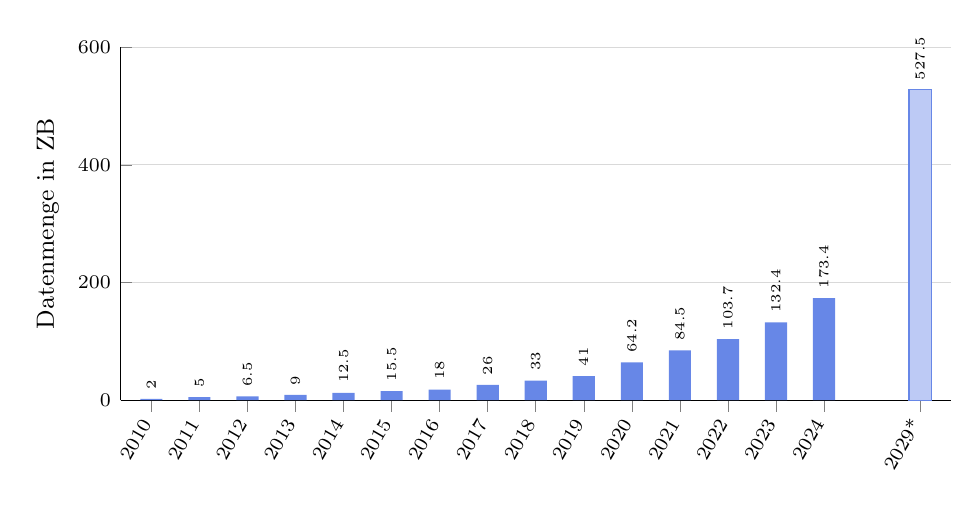
\begin{tikzpicture}
  \begin{axis}[
      width=\linewidth,
      height=.5\linewidth,
      ybar,
      bar width=.8em,
      bar shift=0pt,
      ymin=0, ymax=600,
      ylabel={Datenmenge in ZB},
      % Lücke zwischen 2024 und 2029 als leere Kategorie
      symbolic x coords={2010,2011,2012,2013,2014,2015,2016,2017,2018,2019,2020,2021,2022,2023,2024,gap,2029},
      xtick={2010,2011,2012,2013,2014,2015,2016,2017,2018,2019,2020,2021,2022,2023,2024,2029},
      xticklabels={2010,2011,2012,2013,2014,2015,2016,2017,2018,2019,2020,2021,2022,2023,2024,2029*},
      x tick label style={rotate=60, anchor=east, font=\scriptsize},
      y tick label style={font=\scriptsize},
      ylabel style={font=\small},
      nodes near coords,
      nodes near coords style={font=\tiny, rotate=90, anchor=west},
      point meta=explicit symbolic,
      ymajorgrids, grid style={gray!30},
      axis x line*=bottom, axis y line*=left,
      enlarge x limits=.04,
    ]
    % gemessene bzw. geschätzte Werte bis 2024
    \addplot[fill=RoyalBlue!80, draw=none] coordinates {
        (2010,2) [2] (2011,5) [5] (2012,6.5) [6.5] (2013,9) [9] (2014,12.5) [12.5]
        (2015,15.5) [15.5] (2016,18) [18] (2017,26) [26] (2018,33) [33] (2019,41) [41]
        (2020,64.2) [64.2] (2021,84.5) [84.5] (2022,103.66) [103.7] (2023,132.4) [132.4] (2024,173.4) [173.4]
      };
    % Prognose 2029 (heller dargestellt)
    \addplot[fill=RoyalBlue!35, draw=RoyalBlue!80] coordinates {(2029,527.5) [527.5]};
  \end{axis}
\end{tikzpicture}
}
  \end{figure}
  {\tiny Daten: IDC, veröffentlicht von Western Digital, zusammengestellt von Statista,\\ \url{https://de.statista.com/statistik/daten/studie/267974/umfrage/prognose-zum-weltweit-generierten-datenvolumen/} (abgerufen am 22.11.2026)}
\end{frame}

\begin{frame}{Auftrag}{Skript}
  \begin{itemize}
    \item \aufgabebox{Aufgabe 1.1: Bits und Bytes}
  \end{itemize}
\end{frame}

% \begin{frame}[fragile]{Datenbanken}
%  \begin{figure}[H]
%    \centering
%    \begin{tikzpicture}
%      \tikzstyle{c} = [draw, shape=circle, draw=black!20, fill=black!10]
%      \Large
%      %\draw[step=1cm,gray,very thin] (-4,-4) grid (4,4);
%      \node [circle, draw=black!20, fill=black!10, minimum size=.5cm](db) at (0,0) {\faTable};
%      \node [c](l1) at (-3,0) {\emoji{laptop}};
%      \node [c](l2) at (-2,-2) {\emoji{desktop-computer}};
%      \node [c](l3) at (0,-3) {\emoji{laptop}};
%      \node [c](l4) at (2,2) {\emoji{desktop-computer}};
%      \node [c](l5) at (0,3) {\emoji{laptop}};
%      \node [c](l6) at (3,0) {...};
%      \node [c](mp1) at (2,-2) {\emoji{mobile-phone}};
%      \node [c](mp2) at (-2,2) {\emoji{mobile-phone}};
%      \node(legend) at (0,-4) {\normalsize Geräte können Daten zu Datenbank	 \textcolor{blue}{senden} / \textcolor{red}{empfangen}};


%      \foreach \nodeN in {l1,l2,l3,l4,l5,l6,mp1,mp2}{
%          \path[->, red] (db) edge[bend right=10] node [left] {} (\nodeN);
%          \path[->, blue] (\nodeN) edge[bend right=10] node [left] {} (db);
%        }

%    \end{tikzpicture}
%  \end{figure}
% \end{frame}

\newcommand{\ciascheme}[1]{
  % arg: scaling factor (1 for no rescale)
  %

  \begin{figure}[H]
    \centering
    \scalebox{#1}{
      \begin{tikzpicture}[>=latex',node distance=2cm, every edge/.style={draw}, every node/.style={fill=blue!20}]
        \scriptsize
        % Entities
        \node[entity] (cia) at (0,0) {cia};

        % Attributes
        \node[attribute] (name) at (-2,0) {\underline{Name}} edge (cia);
        \node[attribute](region) at (-1.5,1.5) {Region} edge (cia);
        \node[attribute] (flaeche) at (0,2) {Fläche} edge (cia);
        \node[attribute] (einwohner) at (1.5,1.5) {Einwohner} edge (cia);
        \node[attribute] (bip) at (1.5,0) {BIP} edge (cia);
      \end{tikzpicture}
    }
  \end{figure}
}

\begin{frame}[fragile]{Beispiel-Datenbank: \textit{Central Intelligence Agency} (CIA)}
  \begin{table}
    \centering
    \tiny
    \begin{tabular}{lcccc}
      \toprule
      \textbf{Name}    & \textbf{Region} & \makecell{\textbf{Fläche}\\(Tsd. km$^2$)} & \makecell{\textbf{Einwohner}\\(Mio.)} & \makecell{\textbf{BIP}\\(Mrd. USD)} \\
      \midrule
      Afghanistan      & Asien           & 652             & 25.8               & 21.0         \\
      Albanien         & Europa          & 28.7            & 3.49               & 5.6          \\
      Algerien         & Afrika          & 2381.7          & 31.2               & 147.6        \\
      Amerikanische... & Ozeanien        & 0.199           & 0.0654             & 0.15         \\
      Andorra          & Europa          & 0.468           & 0.0668             & 1.2          \\
      Angola           & Afrika          & 1246.7          & 10.1               & 11.6         \\
      Anguilla         & Mittelamerika   & 0.091           & 0.0118             & 0.088        \\
      Antarktik        & Antarktis       & 14000           & 0                  & 0            \\
      Antigua und...   & Mittelamerika   & 0.442           & 0.0664             & 0.524        \\
      Argentinien      & Südamerika      & 2766.9          & 36.9               & 367          \\
      \midrule
      ...              & ...             & ...             & ...                & ...          \\
      \bottomrule
    \end{tabular}
  \end{table}
  \ciascheme{1}
\end{frame}


% Schema einer Tabelle mit hervorgehobener Spalte (rot), Zeile (blau) und Schlüsselattribut
\newcommand{\highlightTable}{
  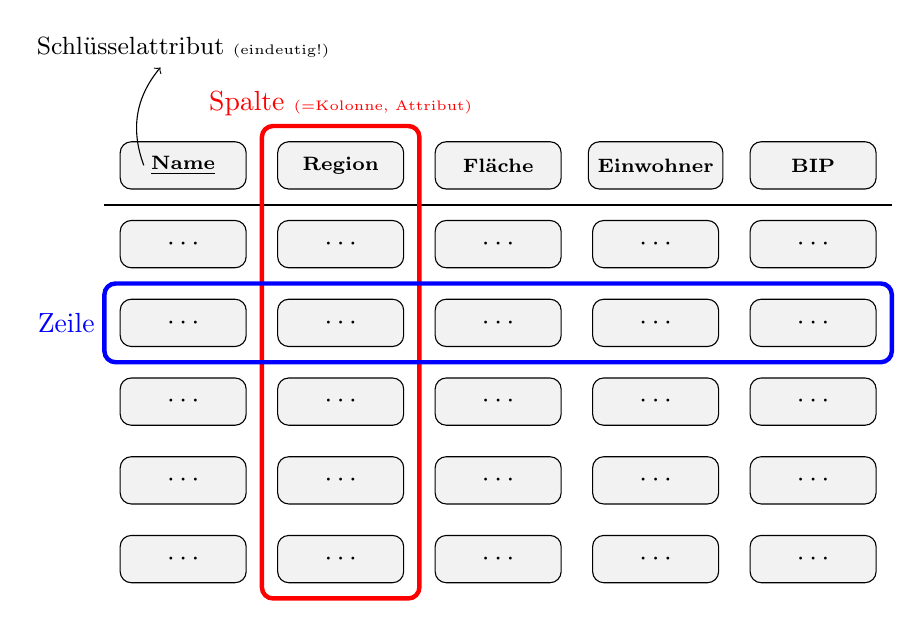
\begin{tikzpicture}
    % Define style for cell
    \tikzstyle{cell} = [draw, rectangle, minimum width=1.6cm, minimum height=.6cm, fill=gray!10, rounded corners]
    \tikzstyle{cellcdot} = [draw, rectangle, minimum width=1.6cm, minimum height=.6cm, fill=gray!0, rounded corners]

    % Draw the table
    \foreach \row in {1,...,6} {
        \foreach \col/\ctitle in {1/\underline{Name},2/Region,3/Fläche,4/Einwohner,5/BIP} {
            \node(\col\row)[cell] at (\col*2, -\row) {
              \ifnum\row=1
                \scriptsize\textbf{\ctitle}\normalsize
              \else
                $\cdots$
              \fi
            };
          }
      }
    \draw[black, thick] (1,-1.5) -- (11,-1.5);

    \draw [red,ultra thick,rounded corners]
    (3,-.5) rectangle (5,-6.5);

    \draw [blue,ultra thick,rounded corners]
    (1,-2.5) rectangle (11,-3.5);

    \node[above] at (4,-0.5){\textcolor{red}{Spalte \tiny(=Kolonne, Attribut)\normalsize}};
    \node[left] at (1,-3){\textcolor{blue}{Zeile}};

    \node(label) at (2,.5) {\small Schlüsselattribut \tiny(eindeutig!)};
    \path[->] (1.5,-1) edge[bend left] node [left] {} (label);
  \end{tikzpicture}
}

\begin{frame}[fragile]{Typische Tabellenstruktur}
  \highlightTable
\end{frame}

\begin{frame}[fragile]{SQL-Befehle}{\lstinline|SELECT [spalten] FROM [tabellenname]|}
  \ciascheme{.7}
  \begin{lstlisting}
SELECT *
FROM cia;
\end{lstlisting}

  \begin{table}
    \centering
    \tiny
    \begin{tabular}{lcccc}
      \toprule
      \textbf{Name}    & \textbf{Region} & \makecell{\textbf{Fläche}\\(Tsd. km$^2$)} & \makecell{\textbf{Einwohner}\\(Mio.)} & \makecell{\textbf{BIP}\\(Mrd. USD)} \\
      \midrule
      Afghanistan      & Asien           & 652             & 25.8               & 21.0         \\
      Albanien         & Europa          & 28.7            & 3.49               & 5.6          \\
      Algerien         & Afrika          & 2381.7          & 31.2               & 147.6        \\
      Amerikanische... & Ozeanien        & 0.199           & 0.0654             & 0.15         \\
      Andorra          & Europa          & 0.468           & 0.0668             & 1.2          \\
      Angola           & Afrika          & 1246.7          & 10.1               & 11.6         \\
      Anguilla         & Mittelamerika   & 0.091           & 0.0118             & 0.088        \\
      Antarktik        & Antarktis       & 14000           & 0                  & 0            \\
      Antigua und...   & Mittelamerika   & 0.442           & 0.0664             & 0.524        \\
      Argentinien      & Südamerika      & 2766.9          & 36.9               & 367          \\
      \midrule
      ...              & ...             & ...             & ...                & ...          \\
      \bottomrule
    \end{tabular}
  \end{table}
\end{frame}

\begin{frame}[fragile]{SQL-Befehle}{\lstinline|SELECT [spalten] FROM [tabellenname]|}
 \ciascheme{.7}
 \begin{lstlisting}
SELECT Name, Region
FROM cia;
\end{lstlisting}

 \begin{table}
   \centering
   \tiny
   \begin{tabular}{lc}
     \toprule
     \textbf{Name}    & \textbf{Region} \\
     \midrule
     Afghanistan      & Asien           \\
     Albanien         & Europa          \\
     Algerien         & Afrika          \\
     Amerikanische... & Ozeanien        \\
     Andorra          & Europa          \\
     Angola           & Afrika          \\
     Anguilla         & Mittelamerika   \\
     Antarktik        & Antarktis       \\
     Antigua und...   & Mittelamerika   \\
     Argentinien      & Südamerika      \\
     \midrule
     ...              & ...             \\
     \bottomrule
   \end{tabular}
 \end{table}
\end{frame}

\begin{frame}[fragile]{SQL-Befehle}{\lstinline|SELECT [spalten] FROM [tabellenname] WHERE [conditions]|}
  \ciascheme{.5}
  \begin{lstlisting}
SELECT Name, Region
FROM cia
WHERE Region = 'Afrika';
\end{lstlisting}

  \begin{columns}[c]
    \centering
    \begin{column}{.3\textwidth}
      \begin{table}
        \centering
        \tiny
        \begin{tabular}{lc}
          \toprule
          \textbf{Name}                & \textbf{Region} \\
          \midrule
          Afghanistan                  & Asien           \\
          Albanien                     & Europa          \\
          \rowcolor[gray]{.8} Algerien & Afrika          \\
          Amerikanische...             & Ozeanien        \\
          Andorra                      & Europa          \\
          \rowcolor[gray]{.8} Angola   & Afrika          \\
          Anguilla                     & Mittelamerika   \\
          Antarktik                    & Antarktis       \\
          Antigua und...               & Mittelamerika   \\
          Argentinien                  & Südamerika      \\
          \midrule
          ...                          & ...             \\
          \bottomrule
        \end{tabular}
      \end{table}
    \end{column}
    \begin{column}{.01\textwidth}
      $\rightarrow$
    \end{column}
    \begin{column}{.3\textwidth}
      \begin{table}
        \centering
        \tiny
        \begin{tabular}{lc}
          \toprule
          \textbf{Name} & \textbf{Region} \\
          \midrule
          Algerien      & Afrika          \\
          Angola        & Afrika          \\
          Benin         & Afrika          \\
          Botswana      & Afrika          \\
          Burkina Faso  & Afrika          \\
          \midrule
          ...           & ...             \\
          \midrule
          Sudan         & Afrika          \\
          Swaziland     & Afrika          \\
          Tanzania      & Afrika          \\
          Togo          & Afrika          \\
          Tunesien      & Afrika          \\
          \bottomrule
        \end{tabular}
      \end{table}
    \end{column}
  \end{columns}
\end{frame}

%\begin{frame}[fragile]{SQL-Befehle}{Vergleichsoperatoren}
%  \begin{columns}[c]
%    \centering
%    \begin{column}{.35\textwidth}
%      \begin{table}[H]
%        \centering
%        \tiny
%        \begin{tabular}{l|l}
%          \makecell{\textbf{Operator}                \\\textbf{in SQL}} & \makecell{\textbf{Mathematische}\\\textbf{Bedeutung}} \\\midrule
%          \texttt{=}  & gleich ($=$)                 \\
%          \texttt{<>} & ungleich ($\neq$)            \\
%          \texttt{<}  & kleiner als ($<$)            \\
%          \texttt{<=} & kleiner oder gleich ($\leq$) \\
%          \texttt{>}  & grösser als ($>$)            \\
%          \texttt{>=} & grösser oder gleich ($\geq$)
%        \end{tabular}
%      \end{table}
%    \end{column}
%    \begin{column}{.6\textwidth}
%      \scriptsize
%      Selektiere Länder mit mehr als 100 Millionen EinwohnerInnen:
%      \begin{lstlisting}
%SELECT Name, Einwohner
%FROM cia
%WHERE Einwohner > 1E8
%\end{lstlisting}
%      \centering$\downarrow$
%      \begin{table}
%        \centering\tiny
%        \begin{tabular}{lr}
%          \toprule
%          \textbf{Name}                  & \textbf{Einwohner} \\
%          \midrule
%          Bangladesh                     & 129'194'224        \\
%          Brasilien                      & 172'860'370        \\
%          China                          & 1'261'832'482      \\
%          Indien                         & 1'014'003'817      \\
%          Indonesien                     & 224'784'210        \\
%          Japan                          & 126'549'976        \\
%          Mexiko                         & 100'349'766        \\
%          Nigeria                        & 123'337'822        \\
%          Pakistan                       & 141'553'775        \\
%          Russland                       & 146'001'176        \\
%          Vereinigte Staaten von Amerika & 275'562'673        \\
%          \bottomrule
%        \end{tabular}
%      \end{table}
%
%    \end{column}
%  \end{columns}
%\end{frame}

%\fboxsep=.6pt
%\newcommand{\cfbox}[2]{%
%  \colorlet{currentcolor}{.}%
%  {\color{#1}%
%    \fbox{\color{currentcolor}#2}}%
%}
%\begin{frame}[fragile]{SQL-Befehle}{Weitere Abfrage-Möglichkeiten}
%  \begin{lstlisting}[language=SQL, basicstyle=\ttfamily\scriptsize, escapeinside={(*@}{@*)}]
%SELECT Name, BIP
%FROM cia
%WHERE BIP (*@\cfbox{red}{\textcolor{green!40!black}{BETWEEN}}@*) 1E6 (*@\cfbox{red}{\textcolor{green!40!black}{AND}}@*) 1E8
%\end{lstlisting}
%  \begin{lstlisting}[language=SQL, basicstyle=\ttfamily\scriptsize, escapeinside={(*@}{@*)}]
%SELECT Name
%FROM cia
%WHERE Name (*@\cfbox{red}{\textcolor{green!40!black}{LIKE}}@*) '%Vereinigte%'
%\end{lstlisting}
%
%  \begin{lstlisting}[language=SQL, basicstyle=\ttfamily\scriptsize, escapeinside={(*@}{@*)}]
%SELECT Name, Einwohner
%FROM cia
%WHERE Name (*@\cfbox{red}{\textcolor{green!40!black}{IN}}@*) ('Deutschland','Frankreich','Polen')
%\end{lstlisting}
%  ... weitere SQL-Befehle in Cheat-Sheet und Skript
%\end{frame}

\begin{frame}{Auftrag}{InstaHub einrichten, erste Abfragen}
  \begin{itemize}
    \item \aufgabebox{Aufgaben 1.2--1.4 im Skript: InstaHub einrichten}
    \item \aufgabebox{Aufgaben 2.1--2.6 im Skript: \texttt{SELECT} und \texttt{WHERE}}
  \end{itemize}
\end{frame}

\begin{frame}[fragile]{Lehrmittel: Cheat Sheet}
	\begin{figure}[H]
		\centering
		\includegraphics[width=.55\textwidth]{Grundlagen_Info/06_Datenbanken/Figures/Cheatsheet}
	\end{figure}

	\begin{itemize}[<+->]
	\item Viel Eigenständigkeit erwartet
	\item Automatische Lösungsvorschläge auf Moodle
	\item Projekt (in wenigen Wochen): \textit{Murder Mystery}
	\end{itemize}
\end{frame}

\begin{frame}[fragile]{Lehrmittel: Skript}
	\begin{columns}[c]
	\centering
		\begin{column}{.4\linewidth}
			\begin{figure}[H]
				\centering
				\includegraphics[width=\columnwidth,height=.55\textheight,keepaspectratio]{Grundlagen_Info/06_Datenbanken/Figures/titlepage}
			\end{figure}
		\end{column}

		\begin{column}{.6\linewidth}
			Als Ergänzung und Vertiefung zum Cheatsheet, sowie Challenge-Aufgaben
		\end{column}
	\end{columns}
	\vspace{.5cm}

	\begin{itemize}
		\item Arbeit hauptsächlich mit Cheat-Sheets
		\item Feedback ist willkommen!
	\end{itemize}
\end{frame}

\begin{frame}{Auftrag: Eigene Tabellen erstellen \& Abfragen schreiben}{Aufgaben auf Moodle und \textbf{Cheatsheet}}
  \begin{itemize}
    \item \aufgabebox{Moodle 1.1: Daten erstellen, verändern und löschen}
    \item \aufgabebox{Moodle 1.2: Daten abfragen}
    \item \aufgabebox{Moodle 1.3: Lernkontrolle}
    \item \challengebox{Aufgaben 2.7--2.17 im Skript: \texttt{DISTINCT}, \texttt{LIKE}, \texttt{ORDER BY}}
  \end{itemize}
\end{frame}